\section{Local remapping}
\label{sec:remap}

\def\Pi{p_i}
\def\Pii{p_{i-1}}

The local remapping algorithm receives as input the route observed
before the path change, $P(t_{i-1})$, and the radius $r'$ where
\dtrack{} detected a change, i.e., $P(t_i)[r'] \ne P(t_{i-1})[r']$.
Local remapping of this change involves measuring hops on the current
route $\Pi=P(t_i)$, and comparing them with hops on
$\Pii\!=\!P(t_{i-1})$.  A hop is \emph{measured} by sending multiple
probes with systematically varied IP flow-ids, similar to Paris
traceroute's MDA~\cite{veitch09balancer}, to discover the mapping
between interfaces of the measured hop and the hop before it (branch
memberships).

Local remapping operates in two phases:  (i)  locating a $\LCZ$
(\secstr~\ref{sec:remap.locate}), and (ii) remapping it
(\secstr~\ref{sec:remap.local}).  By \emph{locating} a $\LCZ$ we mean
finding a radius $r$ inside it.  If the hop at $r'$ is a changed (added)
hop, then $r'\in\LCZ(r')$ and so $\LCZ(r')$ is already located.


% Local remapping starts from radius $r'$ where the current hop differs
% from the previous one, i.e., $\Pi[r^\prime] \ne
% \Pii[r^\prime]$.  If the hop at radius $r^\prime$ in the current
% route is not contained in the previous route, i.e., $\Pi[r^\prime]
% \notin \Pii$, then radius $r^\prime$ is inside the local change
% zone, no search is necessary, and local remapping proceeds to the next
% phase to locally remap the change (\secstr~\ref{sec:remap.local}).

\subsection{Locating a LCZ}
\label{sec:remap.locate}

Assume for the moment that the only hops which have changed lie in $\LCZ(r')$, so there is
only one $\LCZ$.  By definition if we need to locate it then $r'\ge r_c$.
\figstr~\ref{fig:remap.example} gives an example of this scenario with $r'=6$.
A probe to $r'=6$ detects a path change if the returning packet comes
from interface $I_5$ instead of $\{I_6\} = \Pii[6]$.

To locate the $\LCZ$ we need to find a changed hop.  To do so we perform
a binary search over  $0\le r <r'$.  There are three possible outcomes
and associated conclusions or `rules' for the status of hop $h =\Pi[r]$
found at any $r$ during the search:

%\figstr~\ref{fig:remap.example} shows an example of a path change
%consisting of a single $\LCZ$ where hop $\{I_4\}$ was removed and hops $\{I_8\}$ and $\{I_9\}$
%added.  A probe to $r'=6$ detects a path change as the answer comes
%from $\{I_5\} = \Pi[6]$ instead of $\{I_6\} = \Pii[6]$.

\begin{description}
%
	\item[Rule 1] $h \notin \Pii$ --- conclude $r_d < r <
	r_c$, i.e.~$h$ has changed, and so is inside the local change
	zone.
%
	\item[Rule 2] $h \in \Pii$ and $\Pii\langle h\rangle
	\ne r$ --- conclude $r_c \le r$ since $h$ is unchanged but at
	different radius (hop changes must have occurred upstream).
%
	\item[Rule 3] $h\in \Pii$ and $\Pii\langle h\rangle =
	r$ --- conclude $r \le r_d$ since $h$ is unchanged, no evidence
	of any change upstream, and $\LCZ(r')$ is certainly downstream.
%
\end{description}

The location search initializes variables $r_\mathrm{up} = 0$,
$r_\mathrm{down} = r^\prime$.  At each iteration the hop at radius $r =
(r_\mathrm{up} + r_\mathrm{down})/2$ is measured and the appropriate
`Rule' applied.  Under Rule 3 we set $r_\mathrm{up} = r$; under Rule 2
we set $r_\mathrm{down} = r$.  Rule 1 implies we have located a local
change zone, so the location search is terminated and we proceed to the
actual remapping.



%The algorithm applies the following three rules after measuring hop $h =\Pi[r]$:


% Local remapping initializes $r_\mathrm{up} = 0$ and $r_\mathrm{down} =
% r^\prime$.  At each iteration in the search, local remapping measures
% the hop at radius $r = (r_\mathrm{up} + r_\mathrm{down})/2$ and
% proceeds as follows:

% If the previous route contains the hop at radius $r^\prime$ at a
% different radius $r''$, i.e., $\Pi[r^\prime] = \Pii[r'']$,
% then we have a local path change that added or removed hops to the
% path upstream of $r^\prime$.  \figstr~\ref{fig:remap.example} shows an
% example of one path change where hop $I_4$ was removed and hops $I_8$
% and $I_9$ were added.  A probe to radius six detects a path change as
% the answer comes from $\{I_5\} = \Pi[6]$ instead of $\{I_6\} =
% \Pii[6]$ in the previous route.


\begin{figure}[t] % {{{
\vspace{-7mm}
\begin{center}
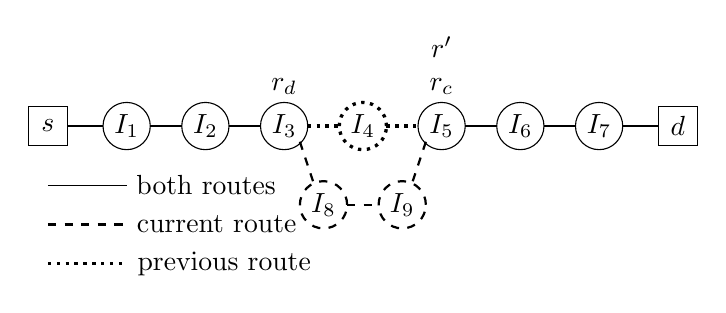
\begin{tikzpicture}
\draw (-2.25,-0.5) -- (-2.25,0) -- (-2.25+0.5,0) -- (-2.25+0.5,-0.5) --
cycle;
\node at (-2,-0.25) {$s$};
%
\draw (6.25-0.5,-0.5) -- (6.25-0.5,0) -- (6.25,0) -- (6.25,-0.5) --
cycle;
\node at (6,-0.25) {$d$};
%
\draw (-1,-0.25) circle (3mm);
\draw (0,-0.25) circle (3mm);
\draw (1,-0.25) circle (3mm);
\draw[dotted, very thick] (2,-0.25) circle (3mm);
%\draw (2,-0.25) circle (3mm);
\draw (3,-0.25) circle (3mm);
\draw (4,-0.25) circle (3mm);
\draw (5,-0.25) circle (3mm);
\node at (-1,-0.25) {$I_1$};
\node at (0,-0.25) {$I_2$};
\node at (1,-0.25) {$I_3$};
\node at (2,-0.25) {$I_4$};
\node at (3,-0.25) {$I_5$};
\node at (4,-0.25) {$I_6$};
\node at (5,-0.25) {$I_7$};
%
\foreach \i in {-1,...,0}
{ \draw (\i+0.3,-0.25) -- (\i+1-0.3,-0.25); }
\foreach \i in {3,...,4}
{ \draw (\i+0.3,-0.25) -- (\i+1-0.3,-0.25); }
\draw[dotted, very thick] (1+0.3,-0.25) -- (2-0.3,-0.25);
\draw[dotted, very thick] (2+0.3,-0.25) -- (3-0.3,-0.25);
\draw (-2.25+0.5,-0.25) -- (-1-0.3,-0.25);
\draw (5+0.3,-0.25) -- (6.25-0.5,-0.25);
%
\draw[dashed, thick] (1.5,-1.25) circle (3mm);
\draw[dashed, thick] (2.5,-1.25) circle (3mm);
\node at (1.5,-1.25) {$I_8$};
\node at (2.5,-1.25) {$I_9$};
\draw[dashed, thick] (1.2,-0.45) -- (1.4,-1.05);
\draw[dashed, thick] (2.8,-0.45) -- (2.6,-1.05);
\draw[dashed, thick] (1.5+0.3,-1.25) -- (2.5-0.3,-1.25);
%
\node at (1, 0.25) {$r_d$};
\node at (3, 0.25) {$r_c$};
\node at (3, 0.75) {$r^\prime$};
%
\draw (-2,-1) -- (-1,-1) node[right] {both routes};
\draw[dashed, thick] (-2,-1.5) -- (-1,-1.5) node[right] {current route};
\draw[dotted, very thick] (-2,-2) -- (-1,-2) node[right] {previous route};
%
\end{tikzpicture}
% \vspace{3cm}
\end{center}
\vspace{-1em}
\caption{Path change removing $I_4$ and adding $I_8$ and $I_9$.}
\label{fig:remap.example}
\end{figure} % }}}

In the general case, where there are other changed hops outside
$\LCZ(r')$, the algorithm may locate another $\LCZ$ to the left of
$\LCZ(r')$ instead of $\LCZ(r')$ itself.

% and looks for hop $\Pi[h]$ on the previous route.
% Again, if hop $\Pi[h]$ is not in the previous route, i.e., $\Pi[h]
% \notin \Pii$, the search finishes and local remapping goes to the
% next phase to remap the change.  If hop $\Pi[h]$ in the current route
% is at radius $h$ in the previous route, i.e., $\Pi[h] =
% \Pii[h]$, then the path change is downstream of $h$ and local
% remapping makes $h_\mathrm{up} = h$.  If hop $\Pi[h]$ is another at
% another radius $h^{\prime\prime}$ in the previous route, i.e.,
% $\Pi[h] = \Pii[h^{\prime\prime}]$, the change is upstream of
% $h$ and local remapping makes $h_\mathrm{down} = h$.

We cannot compare the current route with the previous route if the
router at hop $\Pi[r]$ does not answer probes.  In this case we take a
conservative approach, decrementing $r$ and continuing the search at the
previous hop without updating $r_\mathrm{up}$ and $r_\mathrm{down}$.  If
a path change only removes hops, then all hops in the current route
belong to the previous route.  In this case, the search terminates when
$r_\mathrm{up} = r_\mathrm{down}$.




%%%%%%%%%%%%%%%%%%%%%%%%%%%%%%%%%%%%%%%%%%%%%%%%%%%%%
\subsection{Remapping}
\label{sec:remap.local}

Remapping starts from a radius $r$ of a changed hop inside the located
$\LCZ$, defined by $(r_d,r_c)$.  It sequentially measures hops
downstream of $r$ until it finds the (unchanged) convergence hop
$\Pi[r_c]$.  If one of the branches does not reach $d$, we define the
convergence hop as the last reachable hop, defined as one having three
following unresponsive hops, like in traceroute.  Similarly, local
remapping sequentially measures hops upstream of $r$ as needed until it
finds the (unchanged) divergence hop $\Pi[r_d]$,  terminating at the
source in the worst case.    For path changes that only remove hops, we
have $r_d = r_\mathrm{up} = r_\mathrm{down}=r_c$ at termination and no
remapping is necessary.

The algorithm operates on a principle that it will remap any changes it
becomes aware of in the course of remapping.  Thus if the radius of the
divergence hop $\Pi[r_d]$ has changed, i.e., $r_d \ne \Pii\langle
\Pi[r_d]\rangle$, then this constitutes a detection of other changes, in
particular the existence of another $\LCZ(r_d)$, defined by
$(r_d^1,r_c^1)$ with $r_c^1\le r_d$, upstream of the first.  Similarly,
hops we measured downstream of $r_c$ may have radii incompatible with
the number of hops added or removed by the zone just remapped.  In these
cases, we call the algorithm recursively starting from the radius $r''$
where the new $\LCZ(r'')$ was detected.  This process of remapping
detected changes via $\LCZ$ patches is repeated recursively until there
is no remaining evidence of change.

% \begin{algorithm}[h]
% \caption{Remap phase algorithm (\secstr~\ref{sec:remap.local})
%
% \KwIn{radius $r$ with $r_d < r < r_c$}
%
% % $r_d \leftarrow r$\textbf{,} $r_c \leftarrow r$
%
% % \textbf{while} $\Pi[r_c] \notin \Pii$\textbf{:}
% % $r_c \leftarrow r_c + 1$\textbf{,} measure($r_c$)
%
% % \textbf{while} $\Pi[r_d] \notin \Pii$\textbf{:}
% % $r_d \leftarrow r_d - 1$\textbf{,} measure($r_d$)
%
% \textbf{foreach} $r \in [r_d, r_c]$\textbf{:} measure($r$)
%
% \textbf{if} $r_d \ne \Pii\langle \Pi[r_d]\rangle$\textbf{:}
% search(0, $r_d$)
%
% \textbf{foreach} $r > r_c$ measured\textbf{:}
%
% \Indp
% $h_r \leftarrow \Pi[r]$\textbf{,} $h_c \leftarrow \Pi[r_c]$
%
% \mbox{\textbf{if} $r - r_c \ne \Pii\langle h_r\rangle -
% \Pii\langle h_c\rangle$\textbf{:} search($r_c$, $r$)}
%
% \end{algorithm}



% FIGS. 5--7 FROM SEC. 5
\begin{figure*}
\begin{minipage}{0.33\textwidth}
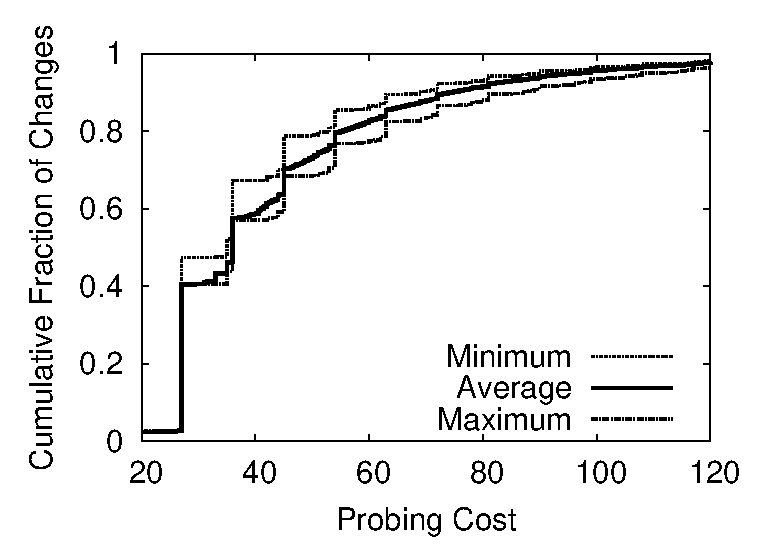
\includegraphics[width=1.05\textwidth]{figs/rmprtcost.eps}
\caption{Probing cost of local remapping over all possible
detection radii.}
\label{fig:sim.rmprt.start}
\end{minipage}
\hfill
\begin{minipage}{0.33\textwidth}
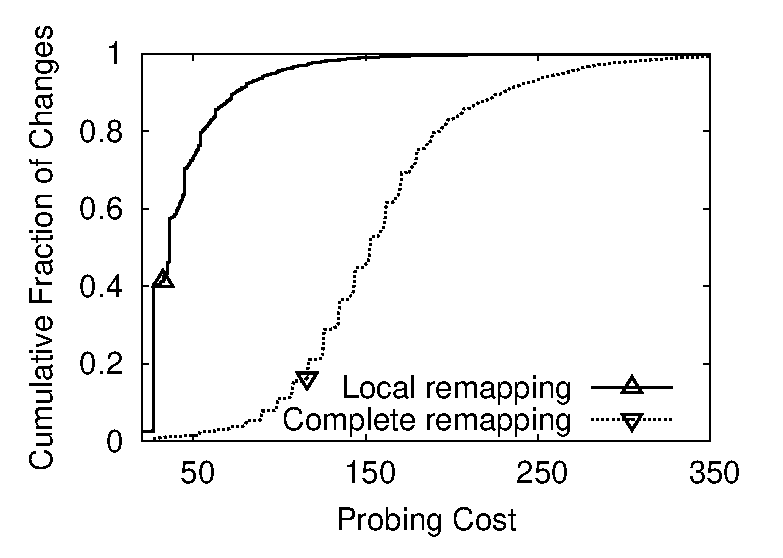
\includegraphics[width=1.05\textwidth]{figs/costprobe.eps}
\caption{Comparing probing cost between local and complete remapping.}
\label{fig:sim.abs.cmp}
\end{minipage}
\hfill
\begin{minipage}{0.33\textwidth}
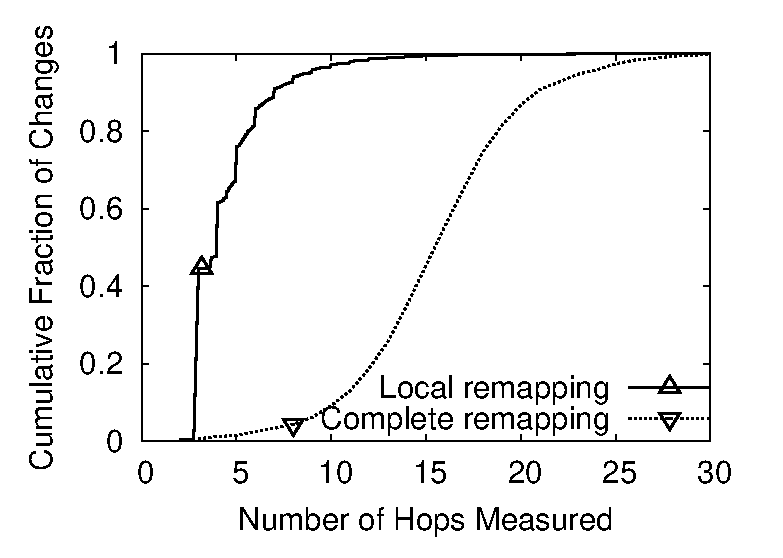
\includegraphics[width=1.05\textwidth]{figs/costhop.eps}
\caption{Comparing number of hops measured during remapping.}
\label{fig:sim.abs.cmp.hops}
\end{minipage}
\end{figure*}


\subsection{Local remapping example}

Consider the path change shown in \figstr~\ref{fig:remap.example}, and
assume it was detected at $r'=6$ as described above.  Since hop $\{I_5\}
=\Pi[r']$ is itself unchanged (existed in $\Pii$), the detection arose
due to the radius being different than expected, 6 instead of 5, and so
$r' \notin \LCZ(r')$ and a location phase is needed.  A binary search is
therefore initiated to locate a change zone.  The search first measures
the hop at $r=r'/2=3$, and finds $\Pii[3] = \Pi[3] = \{I_3\}$,
i.e.~unchanged (and with no evidence of further changes upstream),
indicating that $r_d\ge3$.  Hence Rule 3 applies, and the search then measures
the fourth hop to find $\Pi[4] =\{I_8\}$, which is an added hop (not
in $\Pii$).  Rule 1 now applies:  a $\LCZ$ has been located at $r=4$
(with $r_d$ determined to be $r_d=3$).  The algorithm enters the
remapping phase, measures the fifth hop, and terminates having found
$(h_d,h_c)=(3,5)$ for the located $\LCZ$.  In this case the first $\LCZ$
found is $\LCZ(r')$, the only one in this route.



% \subsection{Serious local remapping example}
%
% Assume a detection at $r'=6$. The associated hop is in the old route at a different radius, so a locating phase is needed.
% Measure $r = 3$ where Rule 2 applies.
% Measure $r = 1$, find $\{I_1\}$, Rule 3 applies.
% Measure $r = 2$, find $\{I_2, I_9\}$, Rule 1 applies.
% Go to local remap and set $(r_d r_c)=(1,3)$.  Find that $\Pi[6] = \{I_5, I_8\}$ is inconsistent with
% the $\LCZ$ we have just remapped: the $\LCZ$ reduced the route length by
% one, but the radius of $\{I_5, I_8\}$ \emph{increased} by 1, implying other changes in the middle.
% Call the algorithm recursively with $r_\mathrm{up} = 3$ and $r_\mathrm{down} = 6$.
% Measure $r = 4$, find $\{I_{10}\}$,  Rule 1 applies, terminate location phase and move to remapping.
% Find $r'_d = 3$ and $r'_c = 6$.  \ed{needs a bit more polishing and checking.}
%
% \begin{figure}[t] % {{{
% \begin{center}
% \begin{tikzpicture}
% \draw (-2.25,-0.5) -- (-2.25,0) -- (-2.25+0.5,0) -- (-2.25+0.5,-0.5) --
% cycle;
% \node at (-2,-0.25) {$s$};
% %
% \draw (6.25-0.5,-0.5) -- (6.25-0.5,0) -- (6.25,0) -- (6.25,-0.5) --
% cycle;
% \node at (6,-0.25) {$d$};
% %
% \draw (-1,-0.25) circle (3mm);
% % \draw (0,-0.25) circle (3mm);
% \draw[dotted, very thick] (0,-0.25) circle (3mm);
% % \draw (1,-0.25) circle (3mm);
% \draw[dotted, very thick] (1,-0.25) circle (3mm);
% \draw (2,-0.25) circle (3mm);
% \draw (3,-0.25) ellipse (3mm and 5mm);
% \draw (4,-0.25) circle (3mm);
% \draw (5,-0.25) circle (3mm);
% \node at (-1,-0.25) {$I_1$};
% \node at (0,-0.25) {$I_2$};
% \node at (1,-0.25) {$I_3$};
% \node at (2,-0.25) {$I_4$};
% \node at (3,+0.0) {$I_5$};
% \node at (3,-0.50) {$I_8$};
% \node at (4,-0.25) {$I_6$};
% \node at (5,-0.25) {$I_7$};
% %
% % \foreach \i in {-1,...,0}
% % { \draw (\i+0.3,-0.25) -- (\i+1-0.3,-0.25); }
% \foreach \i in {3,...,4}
% { \draw (\i+0.3,-0.25) -- (\i+1-0.3,-0.25); }
% \draw[dotted, very thick] (-1+0.3,-0.25) -- (0-0.3,-0.25);
% \draw[dotted, very thick] (0+0.3,-0.25) -- (1-0.3,-0.25);
% \draw[dotted, very thick] (1+0.3,-0.25) -- (2-0.3,-0.25);
% \draw[dotted, very thick] (2+0.3,-0.25) -- (3-0.3,-0.25);
% \draw (-2.25+0.5,-0.25) -- (-1-0.3,-0.25);
% \draw (5+0.3,-0.25) -- (6.25-0.5,-0.25);
% %
% % \draw[dashed, thick] (-0.5,-1.25) circle (3mm);
% \draw[dashed, thick] (0.5,-1.25) ellipse (3mm and 5mm);
% \node at (0.5,-1.0) {$I_2$};
% \node at (0.5,-1.5) {$I_9$};
% \draw[dashed, thick] (-0.8,-0.45) -- (0.3,-1.00);
% \draw[dashed, thick] (1.8,-0.45) -- (0.7,-1.00);
% %
% \draw[dashed, thick] (2.2,-1.25) circle (3mm);
% \draw[dashed, thick] (2.6,-2.0) circle (3mm);
% \node at (2.2,-1.25) {$I_{10}$};
% \node at (2.6,-2.00) {$I_{11}$};
% \draw[dashed, thick] (2.0,-0.55) -- (2.1,-0.95);
% \draw[dashed, thick] (2.25,-1.525) -- (2.50,-1.755);
% \draw[dashed, thick] (3,-0.75) -- (2.70,-1.75);
% %
% % \node at (1, 0.25) {$r_d$};
% % \node at (3, 0.25) {$r_c$};
% % \node at (4, 0.25) {$r^\prime$};
% %
% \draw (3.25,-1.0) -- (4.25,-1.0) node[right] {both routes};
% \draw[dashed, thick] (3.25,-1.5) -- (4.25,-1.5) node[right] {current route};
% \draw[dotted, very thick] (3.25,-2.0) -- (4.25,-2.0) node[right] {previous route};
% %
% \end{tikzpicture}
% % \vspace{3cm}
% \end{center}
% \vspace{-1em}
% \caption{More complex path change.}
% \label{fig:remap.seriousexample}
% \end{figure} % }}}

